\item \points{25} {\bf Logistic Regression: Training stability}

In this problem, we will be delving deeper into the workings of logistic
regression. The goal of this problem is to help you develop your skills
debugging machine learning algorithms (which can be very different from
debugging software in general).

\begin{enumerate}

  \item \subquestionpoints{10} \textbf{Coding question}

In lecture we saw the average empirical loss for logistic regression:
\begin{equation*}
	J(\theta)
	= -\frac{1}{\nexp} \sum_{i=1}^\nexp \left(y^{(i)}\log(h_{\theta}(x^{(i)}))
		+  (1 - y^{(i)})\log(1 - h_{\theta}(x^{(i)}))\right),
\end{equation*}
where $y^{(i)} \in \{0, 1\}$, $h_\theta(x) = g(\theta^T x)$ and
$g(z) = 1 / (1 + e^{-z})$.

Implement logistic regression using gradient descent in
\texttt{src/logreg\_stability/logreg.py}.

Starting with $\theta = \vec{0}$, run gradient descent until the updates to
$\theta$ are small: Specifically, train until the first iteration $k$ such
that $\|\theta_{k} - \theta_{k-1}\|_1 < \epsilon$, where
$\epsilon = 1\times 10^{-5}$, or for a maximum of $10^5$ iterations. Then, perform logistic regression on dataset $A$ in \\
\texttt{src/logreg\_stability/ds1\_a.csv}. You can run the code by simply executing
\texttt{python logreg.py} in the \texttt{src/logreg\_stability} directory.

Include a plot of the training data with $x_1$ on the horizontal axis and $x_2$ on the vertical axis.
To visualize the two classes, use a different symbol for examples $x^{(i)}$
with $y^{(i)} = 0$ than for those with $y^{(i)} = 1$. On the same figure, plot the decision boundary
found by logistic regression (i.e., line corresponding to $p(y|x) = 0.5$).

\textbf{Note:} If you want to print the loss during training, you may encounter some numerical instability issues. Recall that the loss function on an example $(x,y)$ is defined as
$$y\log(h_{\theta}(x)) +  (1 - y)\log(1 - h_{\theta}(x)),$$
where $h_\theta(x)=(1+\exp(-x^\top \theta))^{-1}.$ Technically speaking, $h_{\theta}(x)\in(0,1)$ for any $\theta,x\in\R^{d}.$ However, in Python a real number only has finite precision. So it is possible that in your implementation, $h_{\theta}(x)=0$ or $h_{\theta}(x)=1$, which makes the loss function ill-defined. A typical solution to the numerical instability issue is to add a small perturbation. In this case, you can compute the loss function using
$$y\log(h_{\theta}(x) + \epsilon) +  (1 - y)\log(1 - h_{\theta}(x) + \epsilon),$$
instead, where $\epsilon$ is a very small perturbation (for example, $\epsilon=10^{-5}$).


\ifnum\solutions=1 {
  \begin{answer}
\begin{figure}[H]
    \centering
    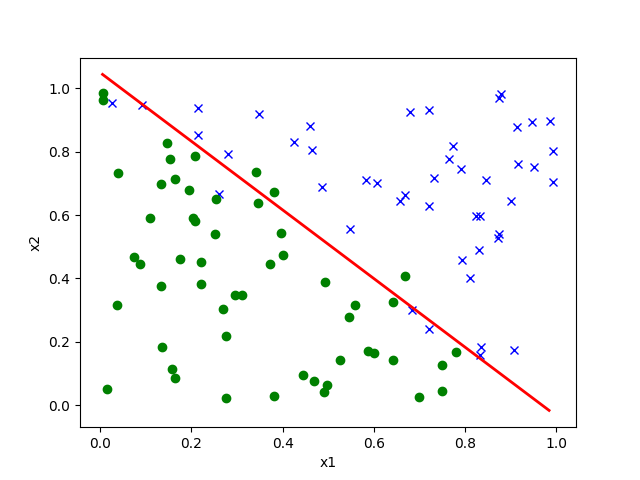
\includegraphics[width=9cm]{logreg_stability/logreg_pred_a.png}
    \caption*{Logistic regression decision boundary on dataset A}
\end{figure}
\end{answer}

} \fi

  \item \subquestionpoints{7}
Perform logistic regression on dataset $B$ in \\
\texttt{src/logreg\_stability/ds1\_a.csv}, and include the same plot as for dataset $A$ in the previous subquestion.
What is the most notable difference in training the logistic regression model
on datasets $A$ and $B$? Investigate why the training procedure behaves unexpectedly on dataset $B$, but
not on $A$. Provide hard evidence (in the form of math, code, plots, etc.) to
corroborate your hypothesis for the misbehavior. Remember, you should address
why your explanation does \emph{not} apply to $A$.

\textbf{Hint}: The issue is not a numerical rounding or over/underflow error.


\ifnum\solutions=1 {
  \begin{answer}
\begin{figure}[H]
    \centering
    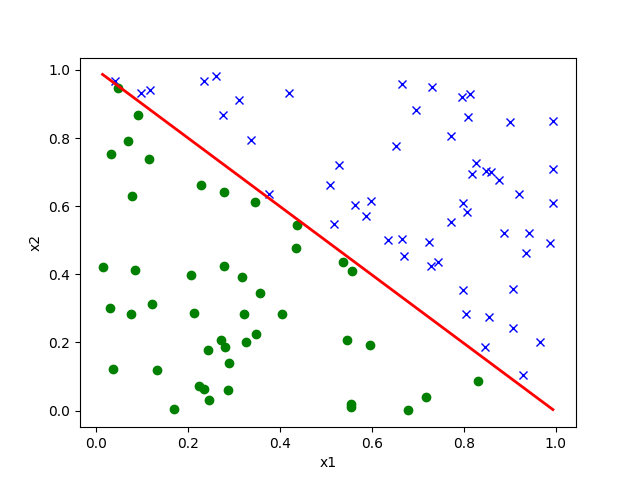
\includegraphics[width=9cm]{logreg_stability/logreg_pred_b.png}
    \caption*{Logistic regression decision boundary on dataset B}
\end{figure}
\begin{figure}[H]
  \centering
  \begin{subfigure}[b]{0.49\textwidth}
    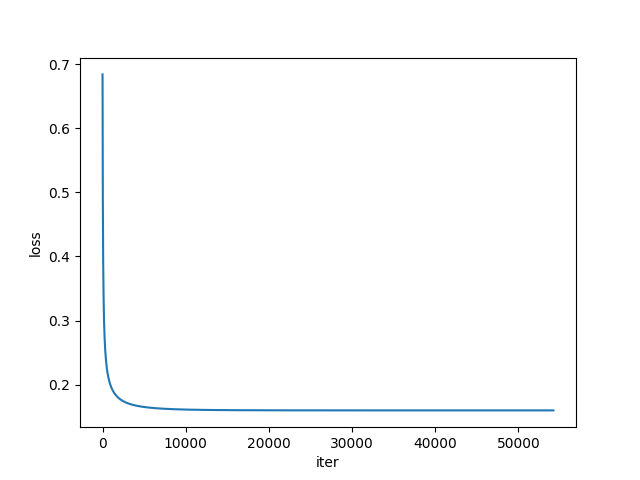
\includegraphics[width=\textwidth]{logreg_stability/logreg_pred_a_loss.png}
    \caption*{Loss by iteration on dataset A}
  \end{subfigure}
  \begin{subfigure}[b]{0.49\textwidth}
    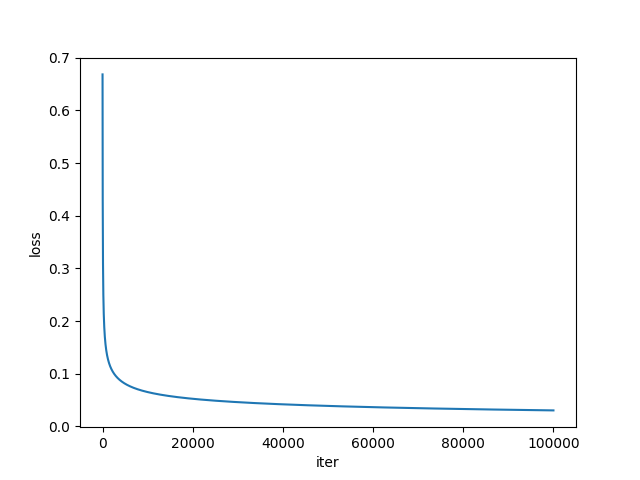
\includegraphics[width=\textwidth]{logreg_stability/logreg_pred_b_loss.png}
    \caption*{Loss by iteration on dataset B}
  \end{subfigure}
\end{figure}
From the decision boundary plot, we observe that dataset B is linearly separable, however by a very small margin. Therefore the the gradient descent doesn't converge, that is due to the weights increasing in magnitude(norm) as the model overfits(model gets overconfident). This phenomenon is displayed on the following plot.
\begin{figure}[H]
  \centering
  \begin{subfigure}[b]{0.49\textwidth}
    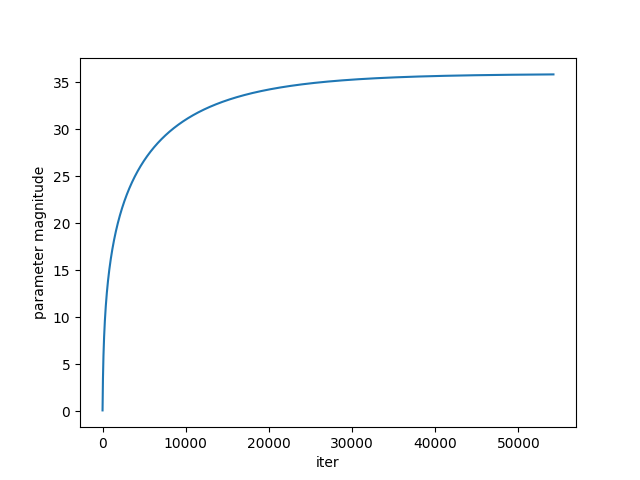
\includegraphics[width=\textwidth]{logreg_stability/logreg_pred_a_param_magnitude.png}
    \caption*{Magnitude of weights for model A}
  \end{subfigure}
  \begin{subfigure}[b]{0.49\textwidth}
    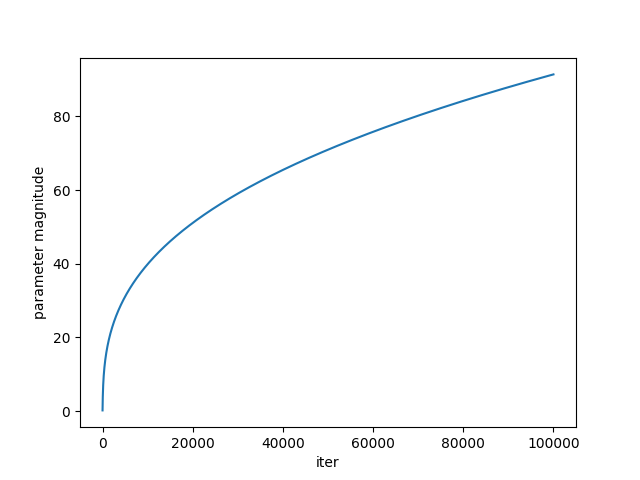
\includegraphics[width=\textwidth]{logreg_stability/logreg_pred_b_param_magnitude.png}
    \caption*{Magnitude of weights for model B}
  \end{subfigure}
\end{figure}
On the plot, we see that the norm of the weights of model B tend to infinity with more iterations.
\end{answer}

} \fi

  \item \subquestionpoints{3}
For each of these possible modifications, state whether or not it would lead to
the provided training algorithm converging on datasets such as $B$. Justify your
answers.
\begin{enumerate}
  \item Using a different constant learning rate.
  \item Decreasing the learning rate over time (e.g. scaling the initial
  learning rate by $1/t^2$, where $t$ is the number of gradient descent
  iterations thus far).
  \item Linear scaling of the input features.
  \item Adding a regularization term $\|\theta\|_2^2$ to the loss function.
  \item Adding zero-mean Gaussian noise to the training data or labels.
\end{enumerate}



\ifnum\solutions=1 {
  \begin{answer}
\begin{enumerate}
  \item As the data is linearly separable, changing the learning rate will only affect how long it takes the model to fit a line that separates the data, it doesn't prevent the model from growing overconfident, therefore the algorithm would not converge.
  \item This will get the algorithm to converge in the sense that the change in norm of weights between iterations will be below the selected $\epsilon$ threshold, however that is only because the learning rate is decaying and not because the model is actually learning. 
  \item After scaling the features, the data is still linearly separable, therefore the algorithm will still not converge 
  \item This prevents the weights from growing and the model getting overconfident. Therefore the algorithm will converge.
  \item Generally this will not work, it depends on the margin of separability. In the case where the data is just barely linearly separable, adding a zero mean Gaussian noise to the training data can make the data not linearly separable, making the algorithm converge. However that is not guaranteed.
\end{enumerate}

\end{answer}

} \fi

  \item \subquestionpoints{5} \textbf{Coding question}
To attempt to fix the issues brought up in the previous subequestions, implement L2 regularization in \texttt{src/logreg\_stability/logreg.py}. Specifically, modify the gradient update to reflect the following loss function:
\begin{equation}
J(\theta)
	= -\frac{1}{\nexp} \sum_{i=1}^\nexp \left(y^{(i)}\log(h_{\theta}(x^{(i)}))
		+  (1 - y^{(i)})\log(1 - h_{\theta}(x^{(i)}))\right) + \frac{1}{2} \lambda \|\theta\|_2^2.
\end{equation}

Run the same code as in the previous subquestion using $\lambda = 0.01$. For both datasets, print the final value of $\theta$, and compare it to the final value of $\theta$ without regularization. Additionally, include a plot of the decision boundary and training data for both datasets and comment on the results qualitatively. How does the decision boundary compare to the one obtained without regularization, especially with respect to the worst misclassified example; in what cases may this be desirable?

\ifnum\solutions=1 {
  \begin{answer}
  \begin{answer}
    \begin{figure}[H]
      \centering
      \vspace{2mm}
      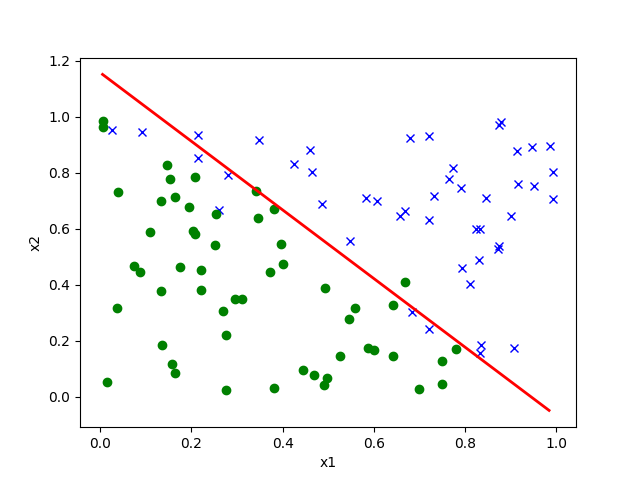
\includegraphics[width=0.65\linewidth]{../src/logreg_stability/logreg_pred_a_reg.png}
          \caption{Separating hyperplane for logistic regression on Dataset 1 with $\lambda = 0.1$}
    \end{figure}

    \begin{figure}[H]
    \centering
    \vspace{2mm}
    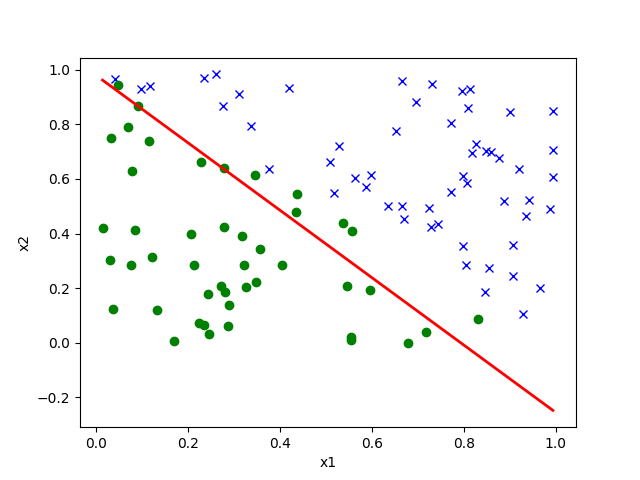
\includegraphics[width=0.65\linewidth]{../src/logreg_stability/logreg_pred_b_reg.png}
    \caption{Separating hyperplane for logistic regression on Dataset 2 with $\lambda = 0.1$}
    \end{figure}

  \end{answer}
\end{answer}

} \fi

\end{enumerate}
